\documentclass{article}
\usepackage{hyperref}
\usepackage[table,xcdraw]{xcolor}
\usepackage{xcolor}
\usepackage{graphicx}
\usepackage{lscape}
\usepackage[francais]{babel}
\usepackage[utf8]{inputenc}
\begin{document}
\title{Rapport de projet Picross}
\author{CONNES Victor \and PRYSIAZHNIUK Anastasiia \and BENAIS-HUGOT Charles \and RIVIERE Cecilie}
\maketitle
\tableofcontents 
\newpage
\section{Description du problème}

Le Picross est un casse-tête qui consiste à retrouver une figure depuis les indices. La figure à découvrir est une grille dans laquelle chaque case est de couleur noire ou blanche. Pour chacune des lignes et colonnes on dispose d'un indice qui est une séquence de nombres représentant les longueurs des blocs de cases noires contigũes de la ligne/colonne. Les blocs de cases noires sont séparés par au moins une case blanche.

\begin{table}[h]
\centering
\begin{tabular}{ccccccc}
\textbf{}  & \textbf{}                       & \textbf{3}                     & \textbf{4}                     & \textbf{4}                     & \textbf{4}                     & \textbf{3}                     \\ \cline{3-7} 
\textbf{2} & \multicolumn{1}{c|}{\textbf{2}} & \multicolumn{1}{c|}{\textbf{}} & \multicolumn{1}{c|}{\textbf{}} & \multicolumn{1}{c|}{\textbf{}} & \multicolumn{1}{c|}{\textbf{}} & \multicolumn{1}{c|}{\textbf{}} \\ \cline{3-7} 
\textbf{}  & \multicolumn{1}{c|}{\textbf{5}} & \multicolumn{1}{c|}{\textbf{}} & \multicolumn{1}{c|}{\textbf{}} & \multicolumn{1}{c|}{\textbf{}} & \multicolumn{1}{c|}{\textbf{}} & \multicolumn{1}{c|}{\textbf{}} \\ \cline{3-7} 
\textbf{}  & \multicolumn{1}{c|}{\textbf{5}} & \multicolumn{1}{c|}{\textbf{}} & \multicolumn{1}{c|}{\textbf{}} & \multicolumn{1}{c|}{\textbf{}} & \multicolumn{1}{c|}{\textbf{}} & \multicolumn{1}{c|}{\textbf{}} \\ \cline{3-7} 
\textbf{}  & \multicolumn{1}{c|}{\textbf{3}} & \multicolumn{1}{c|}{\textbf{}} & \multicolumn{1}{c|}{\textbf{}} & \multicolumn{1}{c|}{\textbf{}} & \multicolumn{1}{c|}{\textbf{}} & \multicolumn{1}{c|}{\textbf{}} \\ \cline{3-7} 
\textbf{}  & \multicolumn{1}{c|}{\textbf{1}} & \multicolumn{1}{c|}{\textbf{}} & \multicolumn{1}{c|}{\textbf{}} & \multicolumn{1}{c|}{\textbf{}} & \multicolumn{1}{c|}{\textbf{}} & \multicolumn{1}{c|}{\textbf{}} \\ \cline{3-7} 
\end{tabular}
\end{table}

\begin{table}[h]
\centering
\begin{tabular}{ccccccc}
\textbf{}  & \textbf{}                       & \textbf{3}                                                                    & \textbf{4}                                                                    & \textbf{4}                                                                    & \textbf{4}                                                                    & \textbf{3}                                                                    \\ \cline{3-7} 
\textbf{2} & \multicolumn{1}{c|}{\textbf{2}} & \multicolumn{1}{c|}{\cellcolor[HTML]{000000}{\color[HTML]{000000} \textbf{}}} & \multicolumn{1}{c|}{\cellcolor[HTML]{000000}\textbf{}}                        & \multicolumn{1}{c|}{\textbf{}}                                                & \multicolumn{1}{c|}{\cellcolor[HTML]{000000}\textbf{}}                        & \multicolumn{1}{c|}{\cellcolor[HTML]{000000}\textbf{}}                        \\ \cline{3-7} 
\textbf{}  & \multicolumn{1}{c|}{\textbf{5}} & \multicolumn{1}{c|}{\cellcolor[HTML]{000000}\textbf{}}                        & \multicolumn{1}{c|}{\cellcolor[HTML]{000000}\textbf{}}                        & \multicolumn{1}{c|}{\cellcolor[HTML]{000000}\textbf{}}                        & \multicolumn{1}{c|}{\cellcolor[HTML]{000000}\textbf{}}                        & \multicolumn{1}{c|}{\cellcolor[HTML]{000000}\textbf{}}                        \\ \cline{3-7} 
\textbf{}  & \multicolumn{1}{c|}{\textbf{5}} & \multicolumn{1}{c|}{\cellcolor[HTML]{000000}{\color[HTML]{000000} \textbf{}}} & \multicolumn{1}{c|}{\cellcolor[HTML]{000000}{\color[HTML]{000000} \textbf{}}} & \multicolumn{1}{c|}{\cellcolor[HTML]{000000}{\color[HTML]{000000} \textbf{}}} & \multicolumn{1}{c|}{\cellcolor[HTML]{000000}{\color[HTML]{000000} \textbf{}}} & \multicolumn{1}{c|}{\cellcolor[HTML]{000000}{\color[HTML]{000000} \textbf{}}} \\ \cline{3-7} 
\textbf{}  & \multicolumn{1}{c|}{\textbf{3}} & \multicolumn{1}{c|}{\textbf{}}                                                & \multicolumn{1}{c|}{\cellcolor[HTML]{000000}\textbf{}}                        & \multicolumn{1}{c|}{\cellcolor[HTML]{000000}\textbf{}}                        & \multicolumn{1}{c|}{\cellcolor[HTML]{000000}\textbf{}}                        & \multicolumn{1}{c|}{\textbf{}}                                                \\ \cline{3-7} 
\textbf{}  & \multicolumn{1}{c|}{\textbf{1}} & \multicolumn{1}{c|}{\textbf{}}                                                & \multicolumn{1}{c|}{\textbf{}}                                                & \multicolumn{1}{c|}{\cellcolor[HTML]{000000}\textbf{}}                        & \multicolumn{1}{c|}{\textbf{}}                                                & \multicolumn{1}{c|}{\textbf{}}   
                                             \\ \cline{3-7} 
\end{tabular}
\caption{Un exemple de Picross et sa solution.}
\end{table}

Certaines grilles peuvent ne pas avoir de solution ou en avoir plusieurs.
\begin{table}[h]
\centering
\begin{tabular}{ccccc}
\textbf{}                       & \textbf{2}            & \textbf{2}            & \textbf{2}            & \textbf{2}            \\ \cline{2-5} 
\multicolumn{1}{c|}{\textbf{2}} & \multicolumn{1}{c|}{} & \multicolumn{1}{c|}{} & \multicolumn{1}{c|}{} & \multicolumn{1}{c|}{} \\ \cline{2-5} 
\multicolumn{1}{c|}{\textbf{2}} & \multicolumn{1}{c|}{} & \multicolumn{1}{c|}{} & \multicolumn{1}{c|}{} & \multicolumn{1}{c|}{} \\ \cline{2-5} 
\multicolumn{1}{c|}{\textbf{2}} & \multicolumn{1}{c|}{} & \multicolumn{1}{c|}{} & \multicolumn{1}{c|}{} & \multicolumn{1}{c|}{} \\ \cline{2-5} 
\multicolumn{1}{l|}{\textbf{2}} & \multicolumn{1}{l|}{} & \multicolumn{1}{l|}{} & \multicolumn{1}{l|}{} & \multicolumn{1}{l|}{} \\ \cline{2-5} 
\end{tabular}
\end{table}

\begin{table}[h]
\centering
\begin{tabular}{ccccc}
\textbf{}                       & \textbf{2}                                    & \textbf{2}                                    & \textbf{2}                                    & \textbf{2}                                    \\ \cline{2-5} 
\multicolumn{1}{c|}{\textbf{2}} & \multicolumn{1}{c|}{}                         & \multicolumn{1}{c|}{}                         & \multicolumn{1}{c|}{\cellcolor[HTML]{000000}} & \multicolumn{1}{c|}{\cellcolor[HTML]{000000}} \\ \cline{2-5} 
\multicolumn{1}{c|}{\textbf{2}} & \multicolumn{1}{c|}{}                         & \multicolumn{1}{c|}{}                         & \multicolumn{1}{c|}{\cellcolor[HTML]{000000}} & \multicolumn{1}{c|}{\cellcolor[HTML]{000000}} \\ \cline{2-5} 
\multicolumn{1}{c|}{\textbf{2}} & \multicolumn{1}{c|}{\cellcolor[HTML]{000000}} & \multicolumn{1}{c|}{\cellcolor[HTML]{000000}} & \multicolumn{1}{c|}{}                         & \multicolumn{1}{c|}{}                         \\ \cline{2-5} 
\multicolumn{1}{l|}{\textbf{2}} & \multicolumn{1}{l|}{\cellcolor[HTML]{000000}} & \multicolumn{1}{l|}{\cellcolor[HTML]{000000}} & \multicolumn{1}{l|}{}                         & \multicolumn{1}{l|}{}                         \\ \cline{2-5} 
\end{tabular}
\end{table}
\newpage

\begin{table}[h]
\centering
\begin{tabular}{ccccc}
\textbf{}                       & \textbf{2}                                    & \textbf{2}                                    & \textbf{2}                                    & \textbf{2}                                    \\ \cline{2-5} 
\multicolumn{1}{c|}{\textbf{2}} & \multicolumn{1}{c|}{\cellcolor[HTML]{000000}} & \multicolumn{1}{c|}{\cellcolor[HTML]{000000}} & \multicolumn{1}{c|}{}                         & \multicolumn{1}{c|}{}                         \\ \cline{2-5} 
\multicolumn{1}{c|}{\textbf{2}} & \multicolumn{1}{c|}{\cellcolor[HTML]{000000}} & \multicolumn{1}{c|}{\cellcolor[HTML]{000000}} & \multicolumn{1}{c|}{}                         & \multicolumn{1}{c|}{}                         \\ \cline{2-5} 
\multicolumn{1}{c|}{\textbf{2}} & \multicolumn{1}{c|}{}                         & \multicolumn{1}{c|}{}                         & \multicolumn{1}{c|}{\cellcolor[HTML]{000000}} & \multicolumn{1}{c|}{\cellcolor[HTML]{000000}} \\ \cline{2-5} 
\multicolumn{1}{l|}{\textbf{2}} & \multicolumn{1}{l|}{}                         & \multicolumn{1}{l|}{}                         & \multicolumn{1}{l|}{\cellcolor[HTML]{000000}} & \multicolumn{1}{l|}{\cellcolor[HTML]{000000}} \\ \cline{2-5} 
\end{tabular}
\caption{Un exemple de Picross qui a deux solutions.}
\end{table}

\begin{table}[h]
\centering
\begin{tabular}{cccccc}
                   &                                 & \textbf{1}            & \textbf{}             & \textbf{}             & \textbf{1}            \\
                   & \textbf{}                       & \textbf{1}            & \textbf{1}            & \textbf{1}            & \textbf{1}            \\ \cline{3-6} 
\textbf{1}         & \multicolumn{1}{c|}{\textbf{1}} & \multicolumn{1}{c|}{} & \multicolumn{1}{c|}{} & \multicolumn{1}{c|}{} & \multicolumn{1}{c|}{} \\ \cline{3-6} 
\textit{\textbf{}} & \multicolumn{1}{c|}{\textbf{3}} & \multicolumn{1}{c|}{} & \multicolumn{1}{c|}{} & \multicolumn{1}{c|}{} & \multicolumn{1}{c|}{} \\ \cline{3-6} 
\textbf{1}         & \multicolumn{1}{c|}{\textbf{1}} & \multicolumn{1}{c|}{} & \multicolumn{1}{c|}{} & \multicolumn{1}{c|}{} & \multicolumn{1}{c|}{} \\ \cline{3-6} 
\end{tabular}
\end{table}

\begin{table}[h]
\centering
\begin{tabular}{cccccc}
                   &                                 & \textbf{1}                                                           & \textbf{}                                     & \textbf{}                                     & \textbf{1}                                                           \\
                   & \textbf{}                       & \textbf{1}                                                           & \textbf{1}                                    & \textbf{1}                                    & \textbf{1}                                                           \\ \cline{3-6} 
\textbf{1}         & \multicolumn{1}{c|}{\textbf{1}} & \multicolumn{1}{c|}{\cellcolor[HTML]{000000}}                        & \multicolumn{1}{c|}{}                         & \multicolumn{1}{c|}{}                         & \multicolumn{1}{c|}{\cellcolor[HTML]{000000}}                        \\ \cline{3-6} 
\textit{\textbf{}} & \multicolumn{1}{c|}{\textbf{3}} & \multicolumn{1}{c|}{\cellcolor[HTML]{C0C0C0}{\color[HTML]{9B9B9B} }} & \multicolumn{1}{c|}{\cellcolor[HTML]{000000}} & \multicolumn{1}{c|}{\cellcolor[HTML]{000000}} & \multicolumn{1}{c|}{\cellcolor[HTML]{C0C0C0}{\color[HTML]{9B9B9B} }} \\ \cline{3-6} 
\textbf{1}         & \multicolumn{1}{c|}{\textbf{1}} & \multicolumn{1}{c|}{\cellcolor[HTML]{000000}}                        & \multicolumn{1}{c|}{}                         & \multicolumn{1}{c|}{}                         & \multicolumn{1}{c|}{\cellcolor[HTML]{000000}}                        \\ \cline{3-6} 
\end{tabular}
\caption{Un exemple de Picross qui n'a pas de solution.}
\end{table}
\newpage


Le but du projet est d'implémenter un solveur de Picross en C++ qui, étant donné une matrice et des indices liés à ses lignes/colonnes, calcule puis affiche sa solution. On ne considère que des Picross qui ont une solution.\newline
La résolution du Picross est un problème NP-complet (en temps Non-déterministe Polynomial). Pour le problème du Picross cela signifie qu'il ne faut pas espérer un algorithme qui résout n'importe quelle grille de Picross avec une complexité polynomiale (en fonction de la taille de la grille), mais trouver une solution peut être beaucoup plus coûteux.

\section{Description de la méthode de résolution utilisée}
Afin de résoudre une grille de Picross donnée, nous traitons ses lignes indépendamment de ses colonnes. 
Le traitement des lignes et des colonnes se faisant de la même manière; nous n'évoquerons par la suite que le traitement des lignes.
\newline
Une première méthode de résolution consisterait à générer toutes les solutions d'une ligne, partiellement remplie ou non; et de déterminer les cases noires ou blanches communes à chacune des solutions.
\newline
Une telle méthode permettrait de déterminer un grand nombre de cases. En revanche, c'est une méthode très coûteuse.
\newline
C'est pourquoi, au lieu de générer toutes les solutions, nous avons choisi d'en générer deux; la plus à gauche et la plus à droite. Cette méthode ne permet pas de déterminer autant de cases que la précédente mais elle est nettement moins coûteuse.
\subsection{La méthode SLG}
La méthode SLG a pour but de générer une solution à une ligne contenant ou non des cases déjà déterminées.
Elle cherchera à placer chacun des blocs de la liste d'indices à partir d'un indice i dans la ligne.
Une fois un bloc placé, elle cherchera à placer le suivant. Si elle n'y parvient pas, elle recommence en i+1.
Afin d'expliciter son fonctionnement, son algorithme est détaillée ci-dessous.
\paragraph{Algorithme : SLG}(L: ligne; n: taille de la ligne; Lind: liste d'indices; i: entier; possible: booleen)
\begin{description}
\item[Debut]
\item[]
  \begin{itemize}
  \item[Si] Lind est vide alors 
    \begin{itemize}
    \item[Si] L ne contient pas de cases noires alors
      \begin{itemize}
      \item possible == vrai;
      \end{itemize}
    \item[Si] possible alors
      \begin{itemize}
      \item on blanchit toutes les cases de L;
      \end{itemize}
    \end{itemize}
  \item[Sinon]
    \begin{itemize}
    \item[Si] l'espace entre i et n est insuffisant pour placer le bloc ou qu'on ne peut pas placer de case blanche apr\`es le bloc ou que l'espace entre i à la taille du bloc contient une case blanche alors
      \begin{itemize}
      \item possible == faux;
      \item On rappelle SLG avec i = i+1;
      \end{itemize}
    \item[Si] possible alors 
      \begin{itemize}
    \item On place le bloc à partir de i;
    \item On rappelle SLG pour l'indice de bloc suivant avec i = i+valeur d'indice précédent+1;
      \end{itemize}
    \end{itemize}
  \end{itemize}
\item[Fin algorithme]
\end{description}
\subsection{Résolution d'une ligne}
\subsubsection{Les méthodes SLPG et SLPD}
Les méthodes SLPG et SLPD génèrent respectivement pour une ligne, sa solution la plus à gauche et sa solution la plus à droite. Elles font toutes deux appel à SLG avec i=0 et possible = faux. 
\newline
Pour la solution droite, SLG est appelé sur une ligne et une liste d'indices préalablement inversées.
\subsubsection{La méthode Fusion}
A la suite des appels à SLPG et SLPD, nous aurons deux solutions possibles pour une ligne; or, pour parvenir à la résolution de notre Picross, il nous faut déterminer les cases n'ayant qu'une solution. 
\newline
Pour ce faire, on fait appel à Fusion qui ne gardera que les cases noires communes aux deux solutions.
Cette dernière nécessite que nos blocs de cases noires soient numérotées (appel à la méthode Numeroter).
\newline
En effet, le status de case noire sûre ne peut être défini que si une case noire commune aux deux solutions appartient à un même et une unique bloc.
\newline
L'exemple ci-dessous illustre l'importance de cette spécification.  
\newline
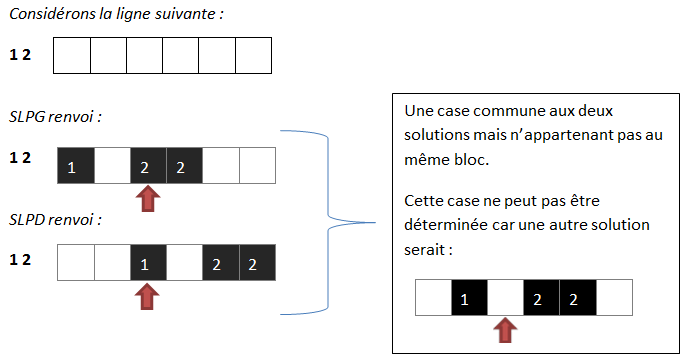
\includegraphics[height=6.5cm,width=12cm]{Exemple1}
\subsubsection{La méthode remplirCasesSureBl}
Cette méthode est appelée après Fusion dans le but de placer les cases blanches sûres. Elle est en mesure de les déterminer grâce aux solutions SLPG-SLPD en calculant les envergures des blocs de cases noires. Dès lors, les espaces situés entre les intervalles trouvés sont des cases blanches sûres.
\paragraph{remplirCasesSureBl} commence par générer une ligne de cases blanche de la même taille que celles prises en paramétre; à savoir, le résultat de Fusion et les solutions SLPG-SLPD; puis ``noircit'' les cases correspantes à l'intervalle qu'occupe chacun des blocs dans l'une et l'autre des solutions SLPG-SLPD.
\newline
A la fin de ce procédé, elle copie les cases blanches restantes dans le résultat de Fusion.
\subsubsection{Ajout de la ligne à la grille de Picross}
Une fois les cases sûres noires et blanches ajoutées à notre ligne, on vérifie par la méthode isFini si elle complète ou non, afin de ne plus la traiter si tel est le cas.
\newline
Ensuite, on ajoute les indices des cases qui ont été modifiées à une liste appelées colModif. Celle-ci permettra de traiter par la suite les colonnes où une case à été ajoutée.
\newline
Pour finir, on recopie notre ligne ainsi complétée dans la grille de Picross.

\subsubsection{la méthode de Backtracking}
A l'aide de nos méthodes précédentes, il peut arriver que des cases ne puissent être déterminées;\newline
Nous avons choisi d'implémenter une méthode de backtracking `simple' qui : 
\begin{itemize}
\item Recherche la 1ere case indeterminée de la matrice (parcours par les lignes)
\item On place cette case à noir
\begin{itemize}
\item On étudie la conséquence de cette coloration arbitraire : 
\begin{itemize}
\item Si cela mène à un picross résolu, on sort
\item Si cela mène à un picross non rempli, on réitère sur une nouvelle case que l'on backtrack
\item Si cela mène à un picross rempli mais non résolu, on sort de nos environnements successifs avec un booléen à false, on effectue alors une recopie de notre matrice qui avait été sauvegardée, et on réitère, cette fois avec la case backtrackée à blanc
\end{itemize}
\end{itemize}
\end{itemize}
\section{Description de l'implémentation}
\subsection{ Les besoins du programme :}

\subsubsection{Pour les indices de chaque ligne/colonne:}
\begin{itemize}
\item Imperatif à satisfaire:
\begin{itemize}
\item structure de taille dynamique (nombre variable d'indices par lignes)
\item parcours en $\theta$(n) (plusieurs méthodes recourant à  un parcours total ou partiel de la structure)
\item relation d'ordre (le parcours ne sont réalisés que dans l'ordre de l'indice le plus en haut vers celui le plus en bas respectivement gauche-droite pour les lignes)
\end{itemize}
\item Choix : la liste simplement chainés, car elle correspond parfaitement au spécification et parait finalement très proche de la réalité
\end{itemize}
\subsubsection{Pour représenter la grille du picross :}
\begin{itemize}
\item Imperatif à satisfaire:
\begin{itemize}
\item structure de taille fixe
\item acc\`es en temps constant a chaque case
\item faciliter de copie de la structure ($\theta$(n))
\end{itemize}
\item Choix: La matrice car très proche de la réalité
\end{itemize}
\subsubsection{Pour l'ensemble des indices de lignes/colonnes :}
\begin{itemize}
\item Imperatif à satisfaire:
\begin{itemize}
\item accéder en temps constant a chaque liste
\item garder un indicage cohérent avec la matrice
\end{itemize}
\item Choix :Un tableau
\end{itemize}
\subsubsection{Pour ligmodif /colmodif}
\begin{itemize}
\item Imperatif à satisfaire:
\begin{itemize}
\item ajout d'un élément en temps constant
\item retrait d'un élément en temps constant
\item taille dynamique
\end{itemize}
\item Choix :
Le choix naturel serait l'ensemble mais on choisit la liste simplement chainés car déjà  implémentés pour les indices de chaque ligne/colonne. Son
comportement est similaire dans le cas d'un ajout et d'un retrait en début de liste .
\end{itemize}
\begin{landscape}
\begin{figure}
\begin{center}
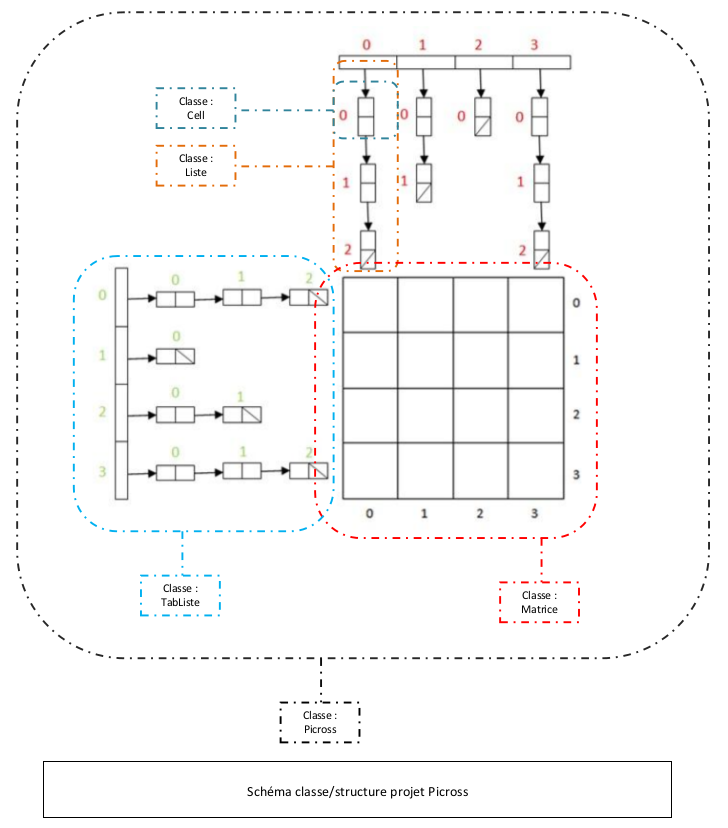
\includegraphics[width=14cm]{./images/recapitulatif_stucture.png}
\end{center}
\end{figure}
\end{landscape}
\newpage
\subsection{ Les classes}
L'ensemble de nos classes disposent d'une surcharge de l'operateur<< afin de faciliter l'affichage dans le terminal. De plus, il existe d'autres classes dans notre programme qui permettent d'améliorer l'affichage en utilisant une interface graphique. Nous ne distinguerons ici seulement les classes permettant la resolution du picross.

\subsubsection{La classe Cell :}
Elle représente un indice logique
\begin{itemize}
\item Attributs :
\begin{itemize}
\item Val : qui représente la valeur de cette indice logique (cette valeur étant strictement enti\`ere positive et a priori non borné nous avons choisi de la représenter par un short int)
\item Suiv : qui est pointeur sur la cellule suivante de la liste
\end{itemize}
\end{itemize}
\subsubsection{La classe Liste :}
\begin{itemize}
\item Attributs :
\begin{itemize}
\item Longueur : qui représente la longueur de la liste. Cette attribut et incrémenter ou décrémenter automatiquement d\`es qu'il y a variations de la taille de la
liste.
\item Fini : Nous indique si la ligne/colonne a laquelle est rattaché la liste est enti\`erement remplie (booléen à  true) ou non (booléen à  false), cette attribut est
notamment tr\`es utile pour vérifier la condition d'arrêt de notre résolution (cf. main)
\item Tête : Pointeur vers le premier élément de la liste.
\end{itemize}
\item Méthode remarquable :
\begin{itemize}
\item Surcharge de l'opérateur() : Nous avons utiliser l'operateur() comme un operateur d'indexage d'une liste cela nous permet notamment de faciliter l'acc\`es
à un element de la liste
\end{itemize}
\end{itemize}
\subsubsection{La classe Tabliste :}
\begin{itemize}
\item Attributs :
\begin{itemize}
\item Tab : le tableau de liste
\item Taille : la taille du tableau
\end{itemize}
\item Méthode remarquable :
\begin{itemize}
\item Surcharge de l'opérateur[]: Nous permet d'utiliser comme si elle était simplement un tableau.
\end{itemize}
\end{itemize}
\subsubsection{La classe Matrice :}
\begin{itemize}
\item Attributs:
\begin{itemize}
\item Tab : la matrice d'entier (-1 : blanc 0 : indéterminé 1 : noir)
\item Nbl : Nombre de ligne
\item Nbc : Nombre de colonnes
\end{itemize}
\end{itemize}
\subsection{ La classe Picross :}
La classe picross est la classe dont les instances représentent les picross; S'est dans cette classe que sont implémenté nos méthodes de résolution.
\subsection{Les algorithmes remarquables :}
\subsubsection{SLG :}
\paragraph{Spécification :}
 void SLG(int*, short int, Cell*, short int, bool\&);
\begin{itemize}
\item Param\`etre:
\begin{itemize}
\item Un tableau d'entier: (Donnée/resultat) il représente une ligne/colonne de notre matrice, initialement il peut contenir des cellules à 1,-1,0
\item Un short int : représentant la taille du tableau
\item Une cellule de liste: il repésente le prochain indice a placer dans le tableau, initialement la première cellule associé à la dite ligne/colonne
\item Un short int : représentant l'indice dans le tableau auquel on souhaite placer le bloc, initialement 0
\item Un booléen passé par référence : représentant si il est possible ou non de placer la fin de la liste d'indices indice courant compté a partir de l'indice courant dans le tableau.
\end{itemize}
\item Retour de la fonction.
\end{itemize}
Le retour ce fait par l'intermédiaire du tableau et du booléen. Si le booléen est à false c'est que le couple (ligne/colonne,liste d'indice) n'a pas de solution. Dans le cas contraire, la solution la plus à gauche nous est donnée dans le tableau.

\paragraph{Complexité pire des cas : $\theta(n^2) <$c$\leq\theta(2^n)$\\ }
 Notons :
\begin{itemize}
\item i: l'indice dans notre tableau
\item n: la taille du dit tableau
\item T: le dit tableau
\item l: la taille de la liste d'indice (le nombre d'indices)
\item $m_i$: l'envergure d'un indice i
\end{itemize}
Dans le pire des cas de notre algorithme, on peut imaginer que chaque hypothèse faite par notre algorithme soit fausse. Pour cela, il nous faut imaginer une liste d'indice de petite taille (ici on choisira $\forall$i $\in$[0,l[ $m_i$=1) en effet, plus les indices sont grands moins ils ont de positions possibles pour une même taille de tableau, et donc moins d'hypothèses.
\newline Enfin, on voit bien que la complexité vas dépendre de la taille de la liste, en effet, chaque cellule appelle la fonction au moins une fois pour chaque maillons placer après dans liste. Au plus, pour un indice j de la liste SLG sera appeé $\sum_{i=l-j}^{l} (i)$ fois c'est à dire l-i fois $\forall$i $\in$[j,l[.
\newline En outre, on sait que le coût de SLG sans les appels récursifs reviens a n puisque dans tous les cas où la liste n'est pas vide, on recopie le tableau. Sinon, si la liste est vide on parcours le tableau de l'indice i à n, ici, on considerera cette valeur cst=n, néanmoins bien que ce cas soit défavorable, il n'est pas réaliste en effet, dans le cas d'une liste non-vide (ce qui est notre cas) alors cette valeur est nécessairement inférieure et decroit tout au long des appels de SLG.
Soit une complexité inférieure à $2^n$.
\newline
Avec ce modèle défavorable on obtient l'équation de recursion suivante:
\begin{center}
 \fbox{SLG(i)= $\sum_{k=l-i}^{l} (SLG(k)*n)+cst$}
\end{center}
Ainsi en notant c la complexité dans ce pire des cas: $\theta(n^2) <$c$\leq\theta(2^n)$, en effet, pour chaque case on parcours au minimun une fois le tableau (la recopie) pour chaque cellule après ici cela fait déjà $\theta(n^2)$ et on doit le faire pour chaque indice.
\paragraph{Complexité meilleur des cas : $\theta$(n)\newline}
Dans le meilleur des cas la liste est vide on doit pacourir une fois le tableau pour pouvoir vérifié.
\subsubsection{Backtrack :}
\paragraph{Spécification :}
 void backtrack(bool \&poss);
\begin{itemize}
\item Param\`etre:
\begin{itemize}
\item Un booléen signalant la possibilité de placer une case dans un picross non fini
\end{itemize}
Dans le cas ou cela est possible, on "backtrack" une case
Dans le cas ou cela n'est pas possible, on revient à l'environnement de la dernière case backtrackée et on l'inverse
\item Retour de la fonction :
\end{itemize}
La fonction ne retourne rien, on travaille directement sur notre Matrice.\newline
Cela à pour conséquence une complexité élevée ($\theta(n^2)$) lors de la recopie de celle-ci.
\subsubsection{Fusion :}
\paragraph{Spécification :}Fusion(int* Merge,int* TG,int* TD,sint taille);
\begin{itemize}
\item Param\`etre:
\begin{itemize}
\item Un tableau d'entier Merge: (Resultat) il représente la ligne/colonne de la matrice,apr\`es la resolution de notre fonction, initialisé avec la ligne/colonne existante
\item Un tableau d'entier TG: (Donnée) il représente la solution la plus à gauche qui résout notre ligne/colonne en fonction de sa liste d'indices et des informations à notre disposition
\item Un tableau d'entier TD: (Donnée) idem pour la solution la plus à droite
\item Un short int taille: représentant la taille du tableau
\end{itemize}
\item Retour de la fonction:
\end{itemize}
La fonction retourne par l'intermédiaire du tableau Merge notre ligne/colonne de depart avec en plus d'éventuelles cases noires "sûres".
\paragraph{Comlexité : $\theta$(n)\newline}
Nous parcourons chaque case du tableau pour vérifier si nous avons des informations supplémentaires. Remarque: on aurait pu gérer une liste des indices qui était encore indéterminé pour chaque ligne/colonne ce qui aurait améliorer notre complexité moyenne. 
Néanmoins, nous avons juger cela peut indispensable au vue du caractère negligeble de cette complexité par rapport aux autres fonctions du programme. 
\subsubsection{remplirCasesSureBl :}
\paragraph{Spécification :}remplirCasesSureBl(int* Merge, int* TG,int* TD, sint taille, Liste \&L);
\begin{itemize}
\item Paramètres:
\begin{itemize}
\item Un tableau d'entier Merge: (Resultat) il représente la ligne/colonne de la matrice,après la résolution de notre fonction, initialisé avec le retour de fusion.
\item Un tableau d'entier TG: (Donnée) il représente la solution la plus à gauche qui résout notre ligne/colonne en fonction de sa liste d'indices et des informations à notre disposition
\item Un tableau d'entier TD: (Donnée) idem pour la solution la plus à droite
\item Un short int taille: représentant la taille du tableau
\item Une liste d'indices L: La liste d'indices associés a la ligne/colonne
\end{itemize}
\item Retour de la fonction:
\end{itemize}
La fonction retourne par l'intermédiaire du tableau Merge notre ligne/colonne de depart avec en plus d'éventuelles case blanches "sures" en se basant sur l'envergure des blocs.
\paragraph{Comlexité : $\theta(n)$\newline}
On doit pour chaque indice de la liste inscrire son envergure dans un tableau intermediaire, pour cela il nous faut parcourir SLG puis SLD mais pas en totalité, en effet, on parcours SLG jusqu'a trouver un indice i1 tel que TG[i1]=0.
On continu notre parcours jusqu'a trouver un indice i2 tel que TG[i2]=0, c'est alors qu'on parcours SLD à partir de i2-1 jusqu'a trouver un indice i3 tel que TG[i3]=0. 
On a alors l'envergure du premier bloc. Pour le deuxiéme on peut commencer notre parcours dans SLG à partir de i2 car il est forcément à droite du premier.\newline 
On trouve alors un nouveau i1 puis un i2 puis un i3 et on recommence alors à partir du nouveau i2 et ainsi de suite. Au final, on aura parcouru entre n et 2n case du tableau.
\subsubsection{remplirCaseBlcoince :}
\paragraph{Spécification :}CaseBlcoince(int* Merge, sint taille, Liste \&L);
\begin{itemize}
\item Param\`etre:
\begin{itemize}
\item Un tableau d'entier Merge: (Resultat) il représente la ligne/colonne de la matrice.
\item Un short int taille: représentant la taille du tableau
\item Une liste d'indices L: La liste d'indices associés a la ligne/colonne
\end{itemize}
\item Retour de la fonction:
\end{itemize}
La fonction retourne par l'intermédiaire du tableau Merge notre ligne/colonne de depart avec en plus d'éventuelles cases blanches "sûres" en se basant sur les tailles des blocs.
\paragraph{Comlexité : $\theta(n)$\newline}

\section{Ameliorations/Evolution du programme:}
\begin{itemize}
\item Dans le cas ou le picross nécessite un backtrack pour sa résolution, les blocs restants peuvent se voir attribuer un degré de liberté, et la case ainsi determinée la plus probable aurait alors été celle choisie pour lancer le backtracking.
\item Dans le souci d'améliorer la compléxitée de la résolution d'une grille en moyenne, nous aurions pû, plutôt que de faire des copies/recopies de matrices entre les environnements de backtrack, ne maintenir que les cases modifiées entre les environnements de backtracks;
Cela dit, dans le pire des cas (aucune case n'est determinable), la complexité reste équivalente ($theta(n^2)$) car l'ensemble des cases se verraient modifiées après le premier environnement de backtrack. (Exemple BT 1 sol)
\item Nous aurions pû implémenter des methodes permettant de rentrer des grilles de picross graphiquement (au clic)
\end{itemize}
\section{Remerciements :}
\begin{itemize}
\item Nous tenions à remercier M.Janssen pour son implication dans le projet, ainsi qu'à l'équipe pédagogique de l'Université.
\end{itemize}
\section{Bibliographie :}
\section{Annexes :}
\end{document}
